\subsection{The controller for the first and second year validation scenario} 
\label{sec:firstSecondValid}
Although the above optimization can handle several control tasks, the control architecture we have been working on is composed of essentially two tasks.
\begin{figure}[t]
    \centering{
    % \includsvg{imgs/model}
        \def\svgwidth{0.2\columnwidth}         
        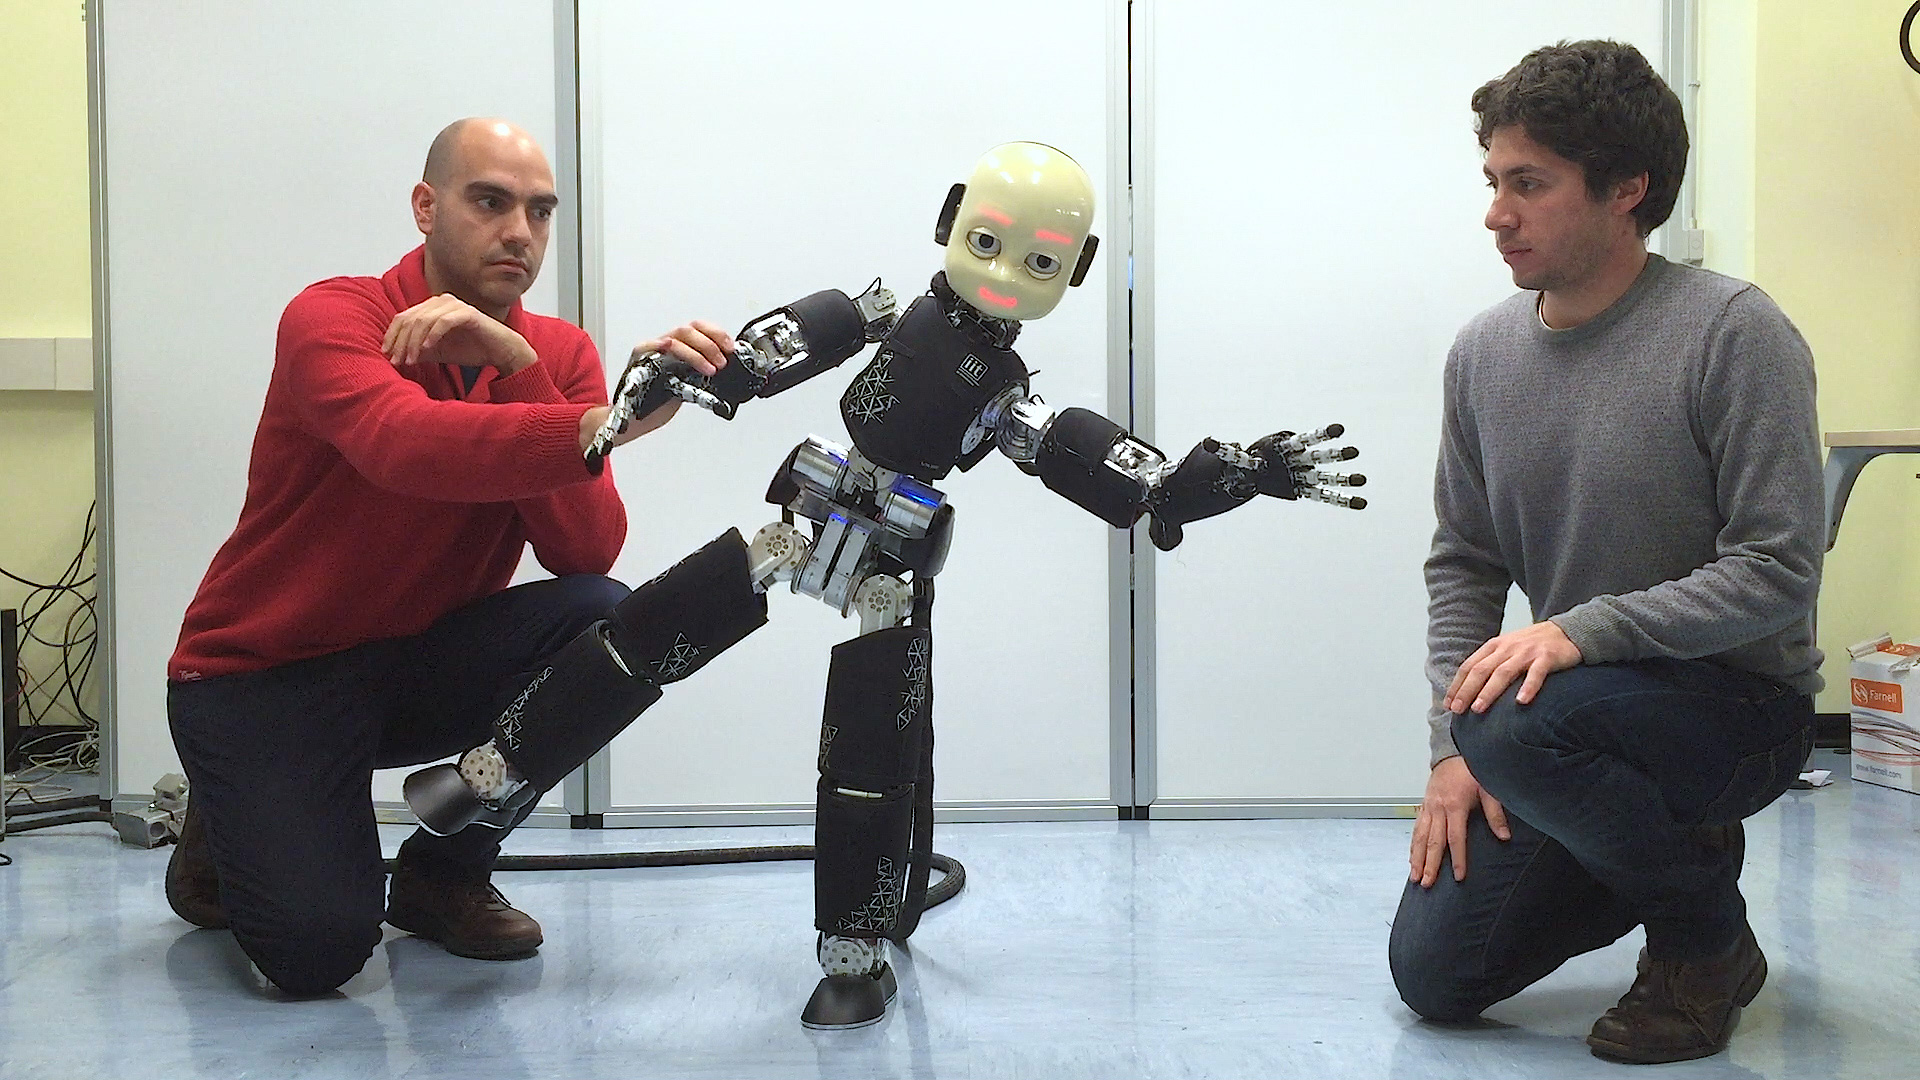
\includegraphics[width=0.65\columnwidth]{images/iCubInteractionOneFoot.jpg}
    \caption{A screen-shot of the one-foot balancing demo }
    \label{fig:oneFootBalnacing}
    }
\end{figure}

\begin{enumerate}
	\item Stabilization of the robot's momentum (expressed at the center-of-mass and with the inertial frame orientation), which is defined by
\begin{IEEEeqnarray}{RCL}
	\yesnumber
	H = \sum H_i = 
	\begin{pmatrix}
	m \dot{x} \\
	H_\omega
	\end{pmatrix},
	\nonumber
\end{IEEEeqnarray}
with $H_i$ the momentum of each link composing the multi-body system, $m$ the total mass of the robot, $x \in \mathbb{R}^3$ the position of the robot center-of-mass, and $H_\omega$ the angular momentum of the multi-body system. 

The control of the robot momentum is achieved assuming the contact wrenches as a virtual control input in the dynamics of $H$. For instance, assuming that the robot is balancing on two feet, two external wrenches $f_L \in \mathbb{R}^6 $ and $f_R \in \mathbb{R}^6$ act on the left and right foot, respectively. Then, one has
\begin{IEEEeqnarray}{RCL}
	\label{centroidalMomentumDyn}
	\yesnumber
	\dot{H} = mg +^c X_L f_L +^c X_R f_R = mg + 
	\begin{pmatrix}
	^c X_L && ^c X_R 
	\end{pmatrix}	
	f,
\end{IEEEeqnarray}
where $^c X_L,^c X_R \in \mathbb{R}^{6\times6}$ are two proper projection matrices, and $f := (f_L^\top,f_R^\top)^\top$.
Since $f$ is assumed to be a control input, one can choose it so that $\dot{H} = \dot{H}^*$, where  $\dot{H}^*$ ensures that $x \rightarrow x_d$ and $H_\omega \rightarrow 0$. Clearly, at this level, one is left with a six-dimensional redundancy of the control input. This redundancy is exploited to minimize joint torques. 
	\item In the null space of the above task, we want the robot to assume a desired joint configuration, while having also some compliance. This is achieved by means of a postural task at the joint torque level, which exploits a proportional-derivative plus gravity compensation control strategy for stabilizing a desired joint reference.
\end{enumerate}

The above control objectives can be formulated as follows. 

\begin{IEEEeqnarray}{RCL}
	\IEEEyesnumber
	\label{optTorque}
	f^* &=& \argmin_{f}  |\tau^*(f)| \IEEEyessubnumber  \\
		   &s.t.& \nonumber \\
		   &&Cf < b \IEEEyessubnumber  \label{frictionCones} \\
		   && \dot{H}(f) = \dot{H}^* \IEEEyessubnumber \label{centroidal} \\
		   &&\tau^*(f) = \argmin_{\tau}  |\tau(f) - \tau_0(f)| 	\label{optPost} 
  \\
		   	&& \quad s.t.  \nonumber \\
		   	&& \quad \quad \ \dot{J}(q,\nu)\nu + J(q)\dot{\nu} = 0
		    \IEEEyessubnumber 	\label{constraintsRigid} \\
		   	&& \quad \quad \ \dot{\nu} = M^{-1}(S\tau+J^\top(q) f - h(q,\nu)) \IEEEyessubnumber \label{acceleration} \\
		   && \quad \quad \ 	\tau_0 = \bar{h}-\bar{J}^{\top}_j f- K_p (q_j-q^{des}_j)- K_d (\dot{q}_j-\dot{q}^{des}_j) \IEEEyessubnumber
		   \yesnumber
\end{IEEEeqnarray}
For the sake of completeness, in the above optimization problem one has
\begin{IEEEeqnarray}{RCL}
	\IEEEyesnumber \\
	 H_d&:=&
\begin{pmatrix}
m\dot{x}_d \\
0
\end{pmatrix}	 \IEEEyesnumber \\
\tilde{H} &:=&H-H_d
\IEEEyessubnumber\\
	\dot{H}^* &=& \dot{H}_d - k_d\tilde{H} -k_p \int_0^t\tilde{H} ds
%	\begin{pmatrix}
%		m(\ddot{x}_d - k_p(x-x_d)-k_d(\dot{x}-\dot{x}_d)) \\
%		-k_\omega H_\omega -k_i \int_0^t  H_\omega ds
%	\end{pmatrix}	 
\IEEEyessubnumber\\
	\bar{h} &:=& h_j - M^\top_{bj}M^{-1}_b h_b \IEEEyessubnumber \\
	\bar{h} &:=& 
	\begin{pmatrix}
	h_b \\ h_j
	\end{pmatrix} =
	{C}(q, {\nu}) {\nu} + {G}(q), \quad h_b \in \mathbb{R}^6 \quad h_j \in \mathbb{R}^n
	 \IEEEyessubnumber \\
	\bar{J} &:=& J_j - J^{\top}_b M^{-1}_b M_{bj} \IEEEyessubnumber	\\
	M &=& 
	\begin{pmatrix}
		M_b && M_{bj} \\
		M^{\top}_{bj} && M_j
	\end{pmatrix}	 \quad M_b \in \mathbb{R}^{6\times 6}
	\quad M_{bj} \in \mathbb{R}^{6\times n}
	\quad M_b \in \mathbb{R}^{n\times n}\IEEEyessubnumber
\end{IEEEeqnarray}

Note that the additional constraint~\eqref{frictionCones} ensures that the desired contact wrenches $f$ belong to the associated friction cones. Once the optimum $f^*$ has been determined, the input torques $\tau$ are obtained by re-using the expression~\eqref{optPost}, i.e.
\begin{IEEEeqnarray}{RCL}
	\label{optTorqueFinal}
	\tau = \tau^*(f^*)
		   \yesnumber
\end{IEEEeqnarray}
By direct calculations one can verify that the solution to the problem~\eqref{optPost} is an affine function versus the desired wrenches $f$, i.e. 
$\tau^* = A(q,\nu)f + b(q,\nu),$
where $A \in \mathbb{R}^{n\times 12}$ and $b \in \mathbb{R}^{n}$ two proper matrices. 
This leads to the following simplification of the optimization problem 
\begin{IEEEeqnarray}{RCL}
	\label{optTorque2}
	\IEEEyesnumber
	f^* &=& \argmin_{f}  |\tau^*(f)|  \IEEEyessubnumber \\
		   &s.t.& \nonumber \\
		   &&Cf < b \IEEEyessubnumber  \label{frictionCones2} \\
		   && \dot{H}(f) = \dot{H}^* \IEEEyessubnumber \\
		   &&\tau^*(f) = A(q,\nu)f + b(q,\nu) \IEEEyessubnumber
		   \yesnumber
\end{IEEEeqnarray}
The above control algorithm has run at both review meetings of the CoDyCo project.

\subsection{Exploiting human-robot interaction  during standing-up motion: passivity based control} 
\begin{figure}
\centering
\begin{subfigure}{.32\textwidth}
  \centering
  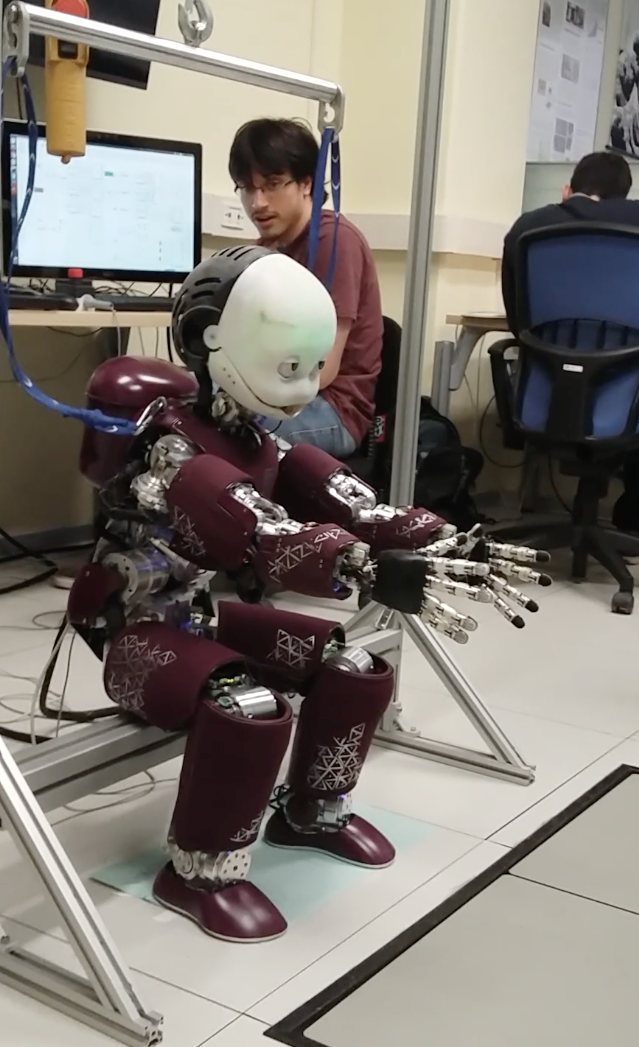
\includegraphics[width=.33\linewidth]{images/icubOnChair.jpg}
  \caption{iCub seating on a bar}
  \label{fig:sub1}
\end{subfigure}%
\begin{subfigure}{.34\textwidth}
  \centering
  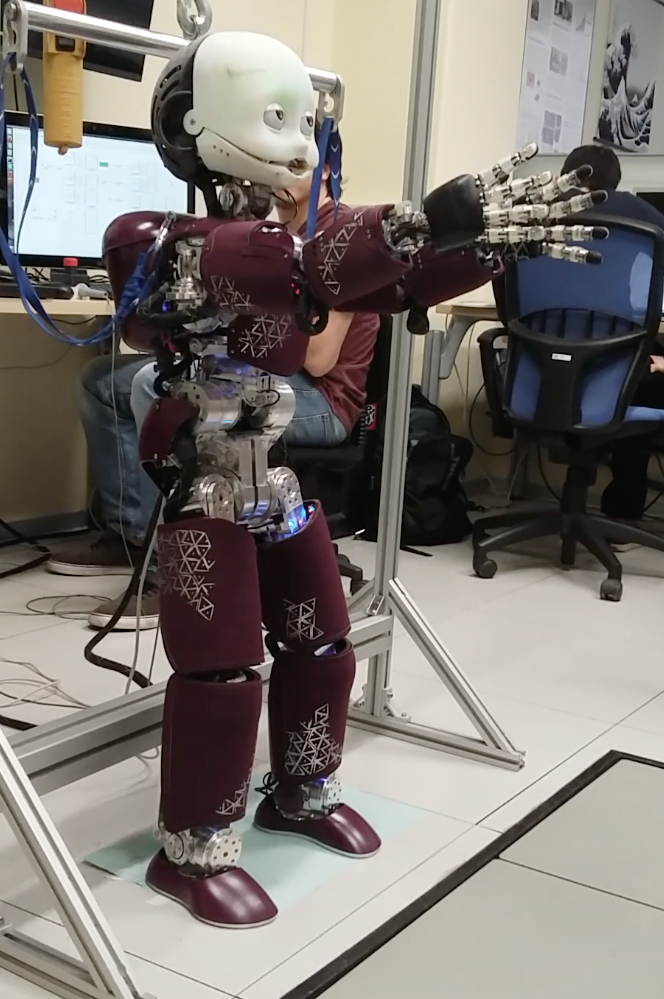
\includegraphics[width=.34\linewidth]{images/iCubUp.jpg}
  \caption{iCub standing on two feet }
  \label{fig:sub2}
\end{subfigure}
\begin{subfigure}{.33\textwidth}
  \centering
  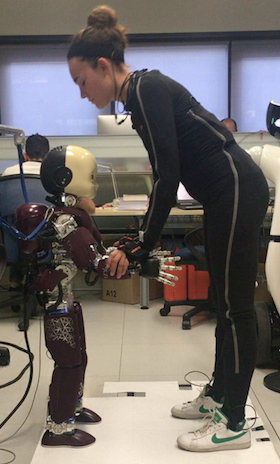
\includegraphics[width=.32\linewidth]{images/icubInteraction.jpg}
  \caption{iCub interacting with users}
  \label{fig:sub3}
\end{subfigure}
\caption{The standing up motion with and without user interaction}
\label{fig:standingUp}
\end{figure}


The controller recalled in the previous section implements on the robot the capacity of stabilising a desired trajectory for the  center-of-mass and a desired joint trajectory. Clearly, both these desired trajectories can be associated with a standing-up motion from the robot being seated on  thighs to the robot standing on two feet, see Figure~\ref{fig:sub1}-\ref{fig:sub2}. A finite state machine coordinates the transitions between these two different robot states by dictating the constraints acting on the system, which in turn characterise  the solutions to the optimisation problem~\eqref{optTorque}. Now, when a user interacts with the robot, it creates external forces on the mechanical system representing it, see Figure~\ref{fig:sub3}. These forces must be taken into account during the standing-up motion in order to make the robot robust against the external perturbations the user creates on the robot. 

Let $F_{ext} \in \mathbb{R}^{n+6}$ denote the torques produced by the external forces acting on the robot. Then,
 assuming that these torques can be measured by means of the force/torque sensors installed within the robot, a very simple way to take into account the external forces is to solve the optimisation problem~\eqref{optTorque} with the constraints~\eqref{centroidal} and~\eqref{acceleration} substituted by:
\begin{IEEEeqnarray}{RCL}
		   	\dot{H}&=&  mg + 
	\begin{pmatrix}
	^c X_L && ^c X_R 
	\end{pmatrix}	
	f + f_{ext}, \IEEEyessubnumber \label{centroidal1}  \\
 	 		\dot{\nu} &=& M^{-1}(S\tau+J^\top(q) f - h(q,\nu)+F_{ext}) \IEEEyessubnumber \label{acceleration1}, 
\end{IEEEeqnarray}
respectively. In the above equation, $f_{ext}\in \mathbb{R}^6$ is the effect of the external wrenches on the centroidal dynamic $\dot{H}$. One of the main problems due to the above approach is that the external wrenches applied on the robot would be completely canceled by the pure feedback linearisation controller associated with this strategy. The macroscopic effect of this cancellation is that if a user would like to \emph{help the robot stand up}, the robot motion would be invariant with respect to the help provided by the user since the effects of the external wrenches are canceled out. So the main question now is:

\vspace{0.5cm}
\noindent
\emph{How can we synthesize a controller that implements the possibility for a user to help the robot lift up during the standing up motion?}
\vspace{0.5cm}

To answer this question, we have to focus on Eq.~\eqref{centroidal1}, and on the role of the fictitious control input $f$ to obtain $\dot{H}(f) = \dot{H}^*$. First, recall that  $\dot{H}^*$, i.e.
\begin{IEEEeqnarray}{RCL}
	\dot{H}^* &=& \dot{H}_d - k_d\tilde{H} -k_p \int_0^t\tilde{H} ds \nonumber
\end{IEEEeqnarray}
renders the energy-based Lyapunov function 
\begin{IEEEeqnarray}{RCL}
	V &=& \frac{1}{2}|\tilde{H}|^2 + \frac{ k_p}{2} \left| \int_0^t\tilde{H} ds  \right | ^2 \label{eq:Lyapuv}
\end{IEEEeqnarray}
negative semi-definite, i.e.
\begin{IEEEeqnarray}{RCL}
	\dot{V} &=& -k_d|\tilde{H}|^2 \label{eq:LyapuvDer}.
\end{IEEEeqnarray}
The equation~\eqref{eq:LyapuvDer} stresses the fact  that an eventual help from a user to lift the robot up is useless: the rate of change of $V$ does not depend upon the external forces, so the standing up motion is invariant to the user interactions. The modification we propose here is based on a decomposition of the external force $f_{ext}$ that highlights the component of this external force that helps decrease the function $V$. More precisely, decompose the external force as follows:
\begin{IEEEeqnarray}{RCL}
	\label{forcedec}
	f_{ext} &=& \alpha\tilde{H}^\parallel + \beta \tilde{H}^\perp \IEEEyessubnumber \label{forcedec1} \\
	\tilde{H}^\parallel  &=&  \frac{\tilde{H}}{|\tilde{H}|}\IEEEyessubnumber \label{forcedec2}  \\
	\alpha &=& \frac{\tilde{H}^\top f_{ext} }{|\tilde{H}|}\IEEEyessubnumber \label{forcedec3}
\end{IEEEeqnarray}
Note that the scalars $\alpha$ and $\beta$ are the components of the external force $f_{ext}$ along and perpendicular to the momentum error $\tilde{H}$. Now, re-define $\dot{H}^*$ as follows 

\begin{equation}
\label{eq:newHStarDot}
  \dot{H}^* =
  \begin{cases}
    \dot{H}_d - k_d\tilde{H} -k_p \int_0^t\tilde{H} ds & \text{if }\quad  \alpha > 0
    \\
   \dot{H}_d - k_d\tilde{H} -k_p \int_0^t\tilde{H} ds +\alpha\tilde{H}^\parallel & \text{if }\quad  \alpha \leq 0
  \end{cases}
\end{equation}
and choose the control input $f$ such that 
\[ \dot{H}(f) = \dot{H}^*. \]
By computing the time derivative of~\eqref{eq:Lyapuv} along the system evolution~\eqref{centroidal1}-\eqref{forcedec}, one easily verifies that:
\begin{equation}
\label{eq:newVDot}
 \dot{V} =-k_d|\tilde{H}|^2 +
  \begin{cases}
   0 & \text{if }\quad  \alpha > 0
    \\
   \alpha|\tilde{H}| & \text{if }\quad  \alpha \leq 0
  \end{cases}
\end{equation}
The fact that when the external forces \emph{help} the robot stand up is encompassed in the right hand side of the above equation:  a negative $\alpha$, i.e. the external forces are in the direction of motion, make the Lyapunov function decrease faster. Hence, we solve the problem~\eqref{optTorque} with~\eqref{eq:newHStarDot} in order to give the possibility of providing help to the robot during standing up motions.